\documentclass{article}\usepackage[]{graphicx}\usepackage[]{color}
%% maxwidth is the original width if it is less than linewidth
%% otherwise use linewidth (to make sure the graphics do not exceed the margin)
\makeatletter
\def\maxwidth{ %
  \ifdim\Gin@nat@width>\linewidth
    \linewidth
  \else
    \Gin@nat@width
  \fi
}
\makeatother

\definecolor{fgcolor}{rgb}{0.345, 0.345, 0.345}
\newcommand{\hlnum}[1]{\textcolor[rgb]{0.686,0.059,0.569}{#1}}%
\newcommand{\hlstr}[1]{\textcolor[rgb]{0.192,0.494,0.8}{#1}}%
\newcommand{\hlcom}[1]{\textcolor[rgb]{0.678,0.584,0.686}{\textit{#1}}}%
\newcommand{\hlopt}[1]{\textcolor[rgb]{0,0,0}{#1}}%
\newcommand{\hlstd}[1]{\textcolor[rgb]{0.345,0.345,0.345}{#1}}%
\newcommand{\hlkwa}[1]{\textcolor[rgb]{0.161,0.373,0.58}{\textbf{#1}}}%
\newcommand{\hlkwb}[1]{\textcolor[rgb]{0.69,0.353,0.396}{#1}}%
\newcommand{\hlkwc}[1]{\textcolor[rgb]{0.333,0.667,0.333}{#1}}%
\newcommand{\hlkwd}[1]{\textcolor[rgb]{0.737,0.353,0.396}{\textbf{#1}}}%

\usepackage{framed}
\makeatletter
\newenvironment{kframe}{%
 \def\at@end@of@kframe{}%
 \ifinner\ifhmode%
  \def\at@end@of@kframe{\end{minipage}}%
  \begin{minipage}{\columnwidth}%
 \fi\fi%
 \def\FrameCommand##1{\hskip\@totalleftmargin \hskip-\fboxsep
 \colorbox{shadecolor}{##1}\hskip-\fboxsep
     % There is no \\@totalrightmargin, so:
     \hskip-\linewidth \hskip-\@totalleftmargin \hskip\columnwidth}%
 \MakeFramed {\advance\hsize-\width
   \@totalleftmargin\z@ \linewidth\hsize
   \@setminipage}}%
 {\par\unskip\endMakeFramed%
 \at@end@of@kframe}
\makeatother

\definecolor{shadecolor}{rgb}{.97, .97, .97}
\definecolor{messagecolor}{rgb}{0, 0, 0}
\definecolor{warningcolor}{rgb}{1, 0, 1}
\definecolor{errorcolor}{rgb}{1, 0, 0}
\newenvironment{knitrout}{}{} % an empty environment to be redefined in TeX

\usepackage{alltt}
\usepackage[sc]{mathpazo}
\usepackage[T1]{fontenc}
\usepackage{geometry}
\geometry{verbose,tmargin=2.5cm,bmargin=2.5cm,lmargin=2.5cm,rmargin=2.5cm}
\setcounter{secnumdepth}{2}
\setcounter{tocdepth}{2}
\usepackage{url}
\usepackage[unicode=true,pdfusetitle,
 bookmarks=true,bookmarksnumbered=true,bookmarksopen=true,bookmarksopenlevel=2,
 breaklinks=false,pdfborder={0 0 1},backref=false,colorlinks=false]
 {hyperref}
\hypersetup{
 pdfstartview={XYZ null null 1}}
\usepackage{breakurl}
\IfFileExists{upquote.sty}{\usepackage{upquote}}{}
\begin{document}


\section*{Problem 2}

\begin{knitrout}
\definecolor{shadecolor}{rgb}{0.969, 0.969, 0.969}\color{fgcolor}\begin{kframe}
\begin{alltt}
\hlcom{# 1). PCA and Kernel PCA to the data}
\hlstd{cancerdata} \hlkwb{<-} \hlkwd{read.table}\hlstd{(}\hlstr{"Cancer.txt"}\hlstd{,} \hlkwc{header} \hlstd{=} \hlnum{FALSE}\hlstd{)}
\hlkwd{names}\hlstd{(cancerdata)} \hlkwb{<-} \hlkwa{NULL}
\hlstd{cancerdata} \hlkwb{<-} \hlkwd{as.matrix}\hlstd{(cancerdata)}
\hlcom{# Due to the computation limitation, I will choose use all of}
\hlcom{# the data to do PCA and use part of data to do kernel PCA.}
\hlstd{prin_cancer} \hlkwb{<-} \hlkwd{prcomp}\hlstd{(cancerdata,} \hlkwc{rtex} \hlstd{=} \hlnum{TRUE}\hlstd{)}
\hlcom{# Check the screeplot of PCA result, it seems that the first}
\hlcom{# principal components contain a large portion of}
\hlcom{# information, which can be used to compress and cluster the}
\hlcom{# data}
\hlkwd{screeplot}\hlstd{(prin_cancer)}
\end{alltt}
\end{kframe}

{\centering 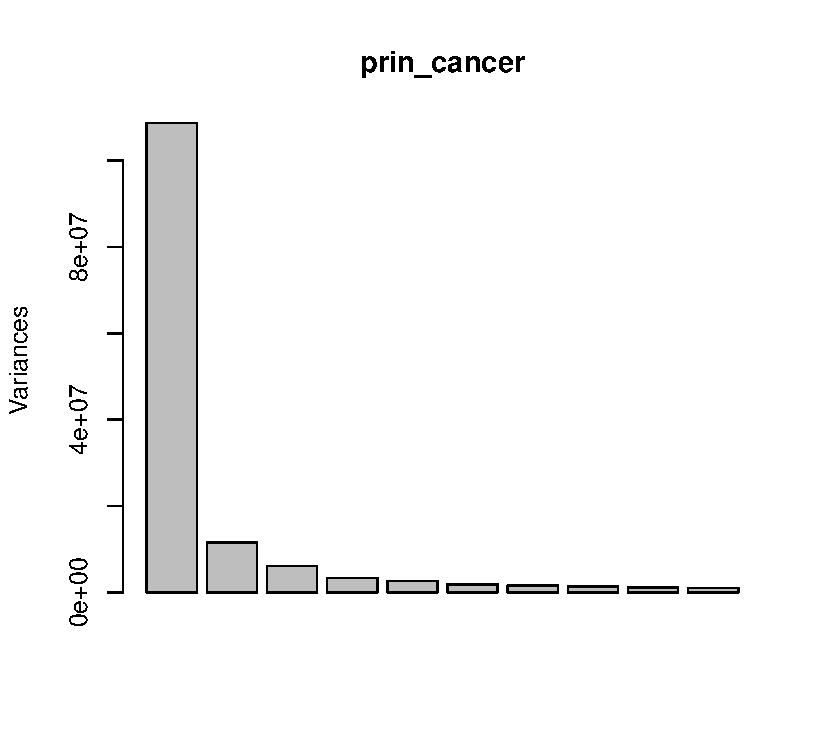
\includegraphics[width=\maxwidth]{figure/minimal-Problem_21} 

}


\begin{kframe}\begin{alltt}
\hlcom{# Then I can plot the projection on the first and second PC}
\hlcom{# loadings, and we can see an obvious clustering of a large}
\hlcom{# portion of data. But we need further investigation in order}
\hlcom{# to find out if we can cluster those points into 14 groups}
\hlcom{# clearly.}
\hlkwd{plot}\hlstd{(prin_cancer}\hlopt{$}\hlstd{x[,} \hlnum{1}\hlstd{], prin_cancer}\hlopt{$}\hlstd{x[,} \hlnum{2}\hlstd{],} \hlkwc{main} \hlstd{=} \hlstr{"Rotated Data from first and second PC direction"}\hlstd{,}
    \hlkwc{xlab} \hlstd{=} \hlstr{"PC_1"}\hlstd{,} \hlkwc{ylab} \hlstd{=} \hlstr{"PC_2"}\hlstd{)}
\end{alltt}
\end{kframe}

{\centering 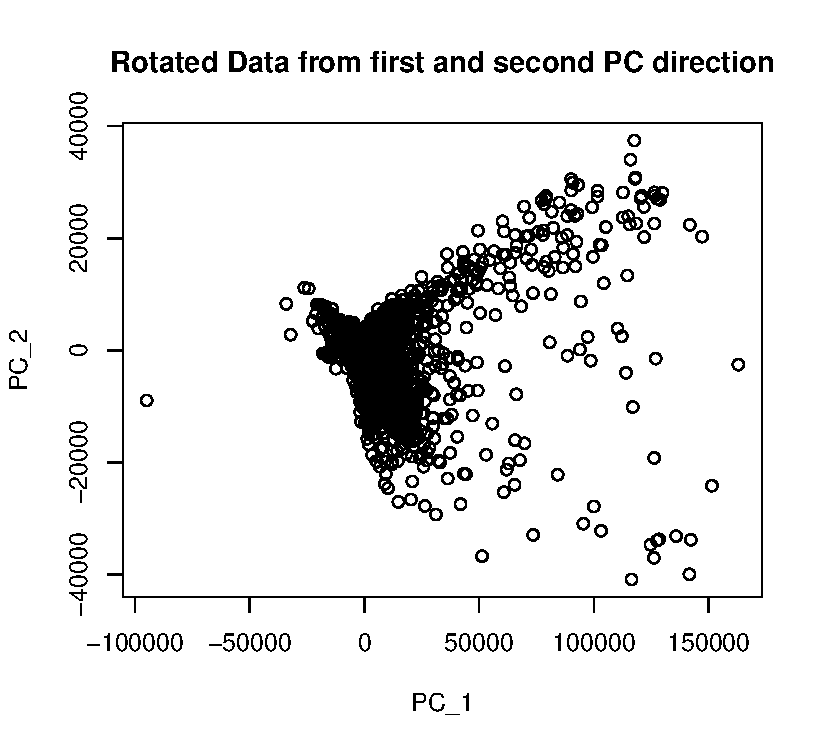
\includegraphics[width=\maxwidth]{figure/minimal-Problem_22} 

}


\begin{kframe}\begin{alltt}
\hlcom{# To further illustrate, I can check the variance}
\hlcom{# contribution of first several principal components.}
\hlstd{explain_var_cancer} \hlkwb{<-} \hlkwd{sapply}\hlstd{(}\hlnum{1}\hlopt{:}\hlnum{144}\hlstd{,} \hlkwa{function}\hlstd{(}\hlkwc{i}\hlstd{)} \hlkwd{sum}\hlstd{(prin_cancer}\hlopt{$}\hlstd{sdev[}\hlnum{1}\hlopt{:}\hlstd{i]}\hlopt{^}\hlnum{2}\hlstd{)}\hlopt{/}\hlkwd{sum}\hlstd{(prin_cancer}\hlopt{$}\hlstd{sdev}\hlopt{^}\hlnum{2}\hlstd{))}
\hlkwd{head}\hlstd{(explain_var_cancer)}  \hlcom{# The first PC contains almost 70% of information.}
\end{alltt}
\begin{verbatim}
## [1] 0.6939 0.7676 0.8068 0.8282 0.8453 0.8568
\end{verbatim}
\begin{alltt}
\hlcom{###### Kernel PCA with Gaussian kernel function ######}
\hlkwd{library}\hlstd{(kernlab)}
\hlstd{rbf} \hlkwb{<-} \hlkwd{rbfdot}\hlstd{(}\hlkwc{sigma} \hlstd{=} \hlnum{0.001}\hlstd{)}
\hlstd{kern_cancer} \hlkwb{<-} \hlkwd{kernelMatrix}\hlstd{(rbf,} \hlkwd{scale}\hlstd{(cancerdata[}\hlnum{1}\hlopt{:}\hlnum{3000}\hlstd{, ]))}  \hlcom{#Part of the data due to computation limit.}
\hlstd{kp_cancer} \hlkwb{<-} \hlkwd{kpca}\hlstd{(kern_cancer)}
\hlcom{# We can check the screeplot of the kernel PCA outcome, it}
\hlcom{# seems we have a really good scree plot and the first and}
\hlcom{# second principal component to project the data.}
\hlkwd{plot}\hlstd{(}\hlkwd{eig}\hlstd{(kp_cancer))}
\end{alltt}
\end{kframe}

{\centering 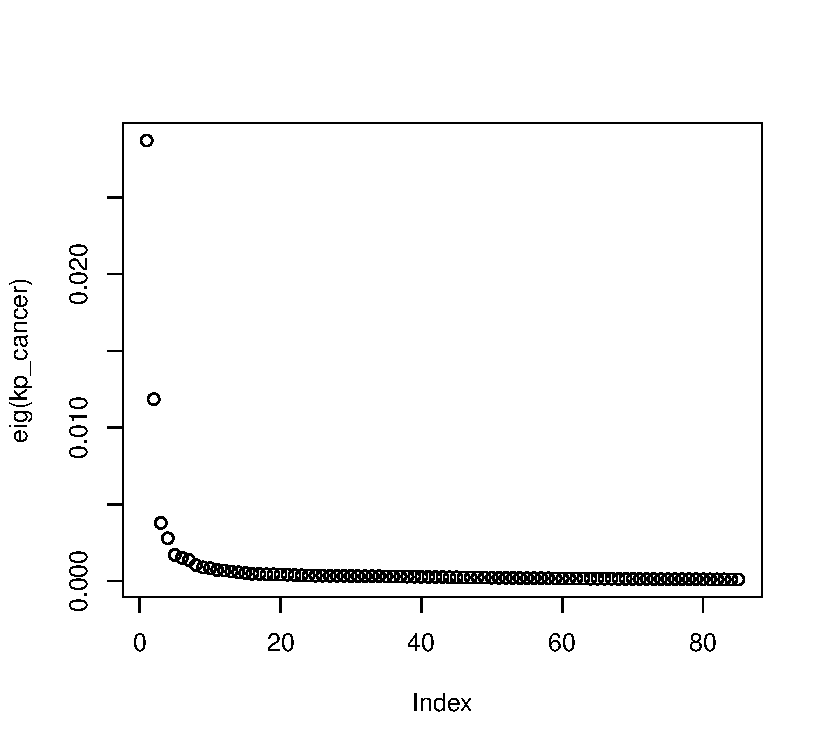
\includegraphics[width=\maxwidth]{figure/minimal-Problem_23} 

}


\begin{kframe}\begin{alltt}
\hlkwd{plot}\hlstd{(}\hlkwd{rotated}\hlstd{(kp_cancer)[,} \hlnum{1}\hlstd{],} \hlkwd{rotated}\hlstd{(kp_cancer)[,} \hlnum{2}\hlstd{],} \hlkwc{main} \hlstd{=} \hlstr{"Rotated Data On First and Second PC direction"}\hlstd{,}
    \hlkwc{xlab} \hlstd{=} \hlstr{"PC_1"}\hlstd{,} \hlkwc{ylab} \hlstd{=} \hlstr{"PC_2"}\hlstd{)}
\end{alltt}
\end{kframe}

{\centering 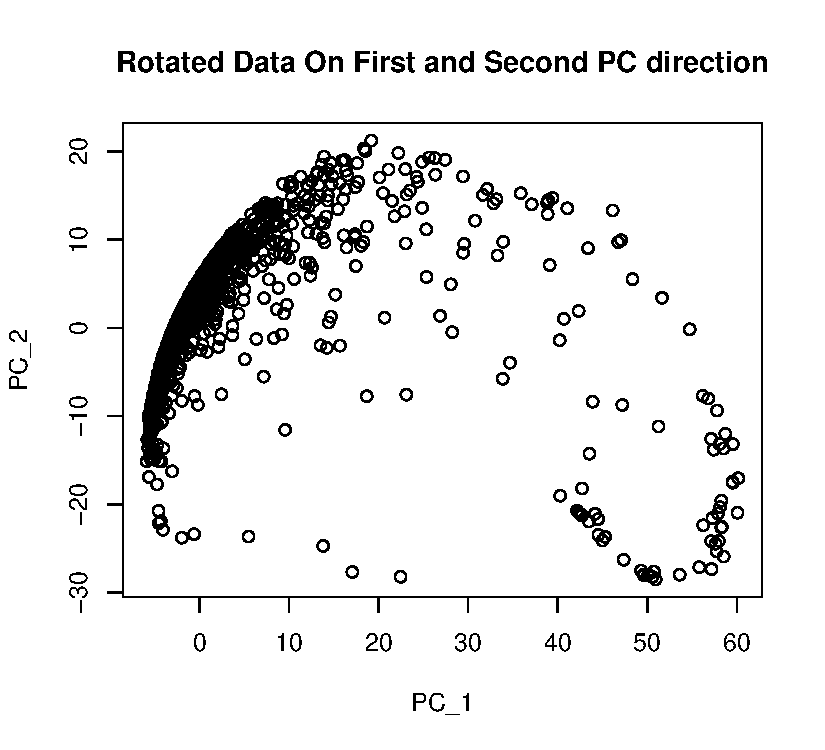
\includegraphics[width=\maxwidth]{figure/minimal-Problem_24} 

}


\begin{kframe}\begin{alltt}
\hlcom{# Comment: we can observe that there are two groups of points}
\hlcom{# emerging, and we would expect to have more groups if we use}
\hlcom{# all of the data.}
\hlcom{# 2).  K-means ###########}
\hlstd{kmean} \hlkwb{<-} \hlkwd{kmeans}\hlstd{(}\hlkwd{t}\hlstd{(cancerdata),} \hlnum{14}\hlstd{,} \hlkwc{nstart} \hlstd{=} \hlnum{1}\hlstd{)}
\hlkwd{plot}\hlstd{(}\hlkwd{t}\hlstd{(cancerdata),} \hlkwc{col} \hlstd{= kmean}\hlopt{$}\hlstd{cluster,} \hlkwc{pch} \hlstd{= kmean}\hlopt{$}\hlstd{cluster,}
    \hlkwc{main} \hlstd{=} \hlstr{"14 clusters using k-means before PCA"}\hlstd{)}
\end{alltt}
\end{kframe}

{\centering 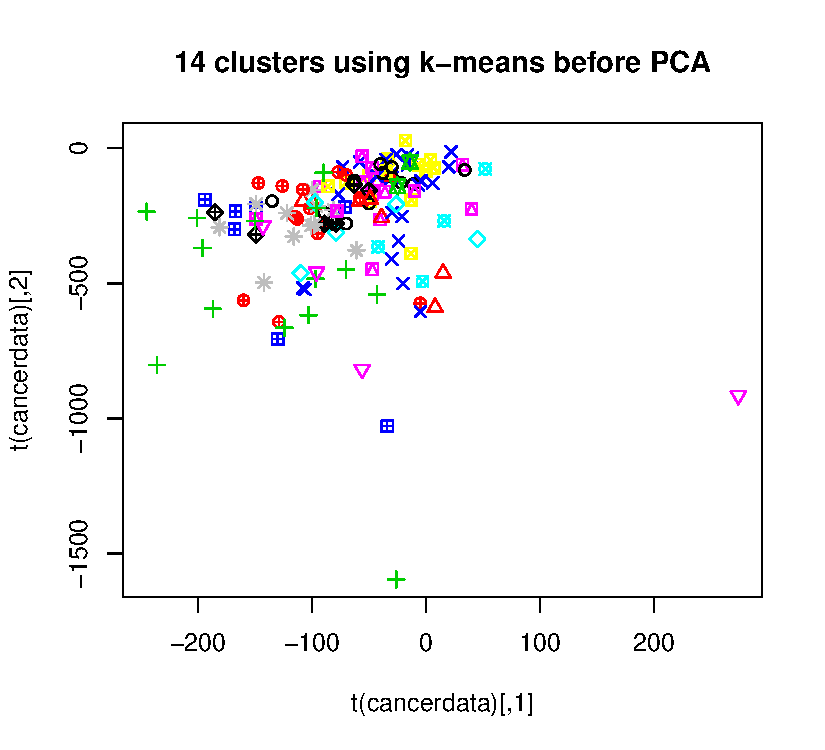
\includegraphics[width=\maxwidth]{figure/minimal-Problem_25} 

}


\begin{kframe}\begin{alltt}
\hlcom{# Comment: K-means does not help us to clearly cluster the}
\hlcom{# datapoints, and we need to figure out better clustering.}
\hlcom{# I use the projected data in the first and second PCs and I}
\hlcom{# expect to have a better clustering outcome.}
\hlstd{kmeans_PCA} \hlkwb{<-} \hlkwd{kmeans}\hlstd{(}\hlkwd{t}\hlstd{(prin_cancer}\hlopt{$}\hlstd{x),} \hlnum{14}\hlstd{,} \hlkwc{nstart} \hlstd{=} \hlnum{1}\hlstd{)}
\hlkwd{plot}\hlstd{(prin_cancer}\hlopt{$}\hlstd{x,} \hlkwc{col} \hlstd{= kmeans_PCA}\hlopt{$}\hlstd{cluster,} \hlkwc{pch} \hlstd{= kmeans_PCA}\hlopt{$}\hlstd{cluster,}
    \hlkwc{main} \hlstd{=} \hlstr{"14 clusters using k-means after normal PCA"}\hlstd{)}
\end{alltt}
\end{kframe}

{\centering 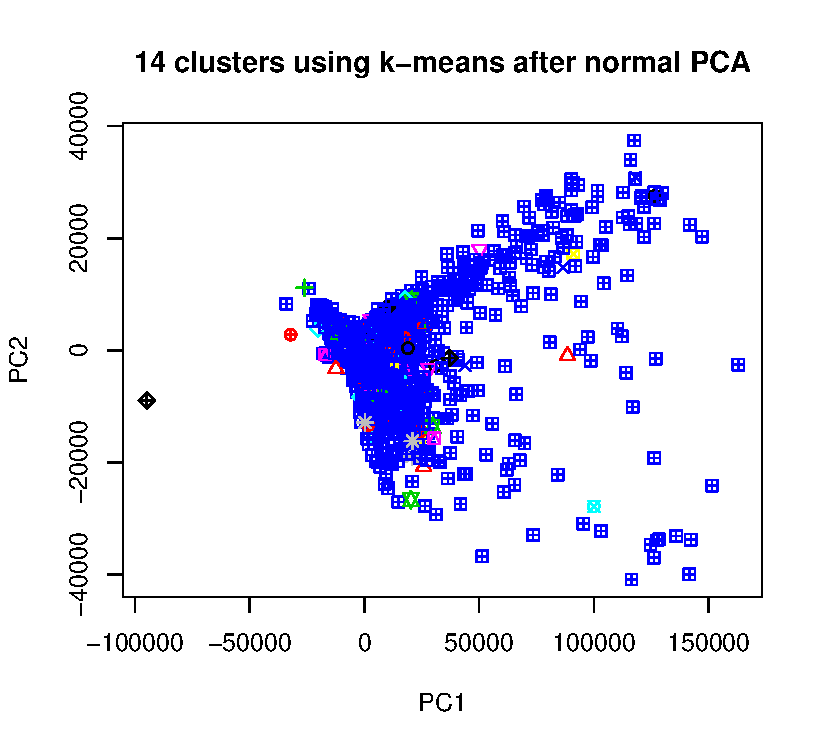
\includegraphics[width=\maxwidth]{figure/minimal-Problem_26} 

}


\begin{kframe}\begin{alltt}
\hlcom{# Comment: we have a majority of points being classfied in}
\hlcom{# one group, it means that PCA does not identify them into}
\hlcom{# different groups, and they have similar variance in most of}
\hlcom{# PC loading directions.}
\hlstd{kmeans_kpca} \hlkwb{<-} \hlkwd{kmeans}\hlstd{(}\hlkwd{t}\hlstd{(}\hlkwd{rotated}\hlstd{(kp_cancer)),} \hlnum{14}\hlstd{,} \hlkwc{nstart} \hlstd{=} \hlnum{1}\hlstd{)}
\hlkwd{plot}\hlstd{(}\hlkwd{rotated}\hlstd{(kp_cancer),} \hlkwc{pch} \hlstd{= kmeans_kpca}\hlopt{$}\hlstd{cluster,} \hlkwc{main} \hlstd{=} \hlstr{"14 clusters using k-means using kernel PCA"}\hlstd{)}
\end{alltt}
\end{kframe}

{\centering 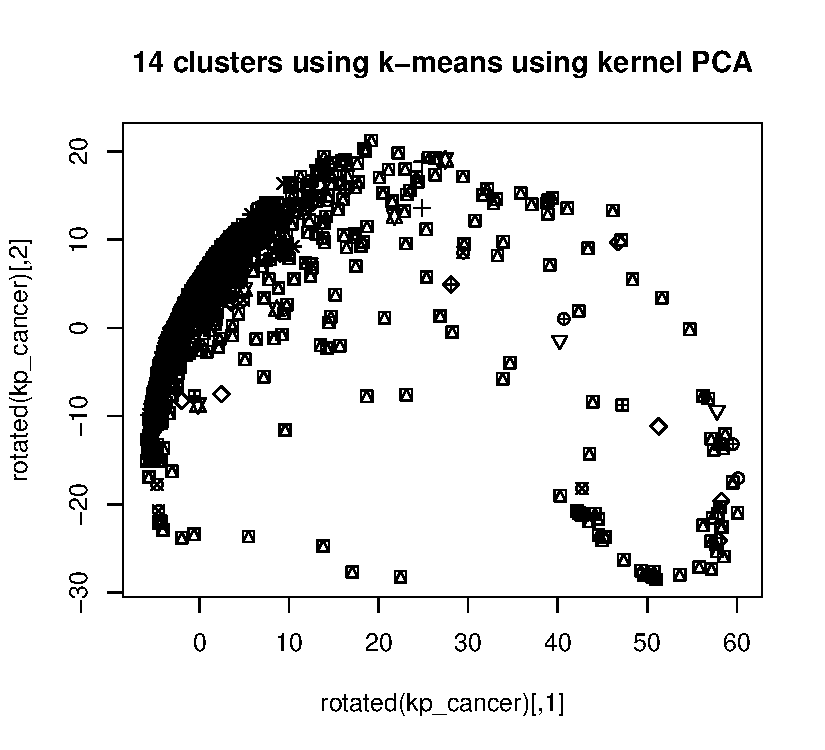
\includegraphics[width=\maxwidth]{figure/minimal-Problem_27} 

}


\begin{kframe}\begin{alltt}
\hlcom{# Comment: Obviously, the k-means method is biased by an}
\hlcom{# outlier.}
\hlcom{####### K-medoids #########}
\hlkwd{library}\hlstd{(cluster)}
\hlstd{diss} \hlkwb{<-} \hlkwd{dist}\hlstd{(}\hlkwd{t}\hlstd{(cancerdata))}
\hlstd{kmedoids} \hlkwb{<-} \hlkwd{pam}\hlstd{(diss,} \hlnum{14}\hlstd{,} \hlkwc{do.swap} \hlstd{=} \hlnum{FALSE}\hlstd{)}
\hlkwd{plot}\hlstd{(cancerdata,} \hlkwc{col} \hlstd{= kmedoids}\hlopt{$}\hlstd{cluster,} \hlkwc{pch} \hlstd{= kmedoids}\hlopt{$}\hlstd{cluster,}
    \hlkwc{main} \hlstd{=} \hlstr{"K-mediods clustering before PCA"}\hlstd{)}
\end{alltt}
\end{kframe}

{\centering 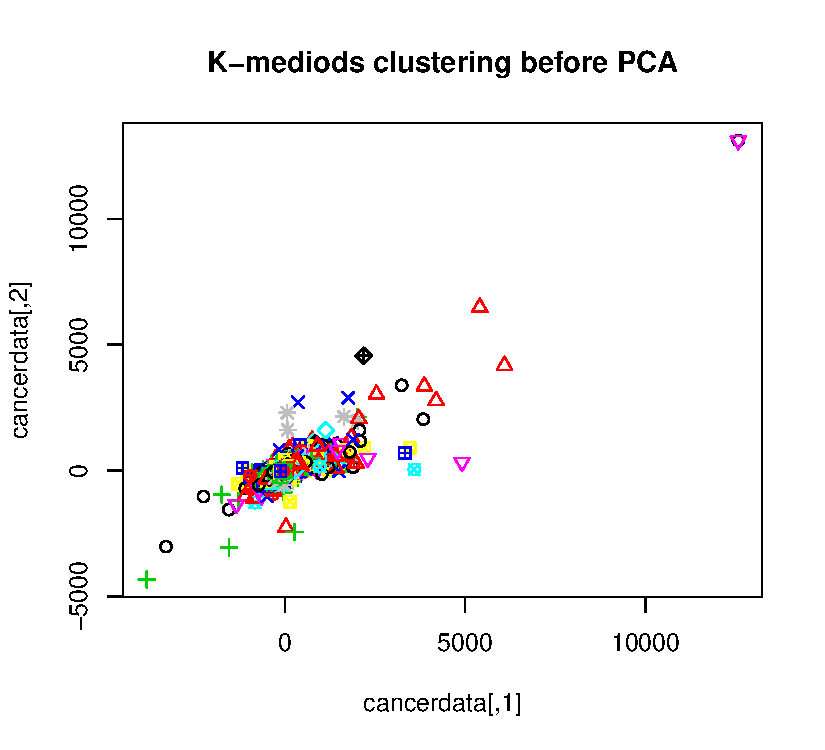
\includegraphics[width=\maxwidth]{figure/minimal-Problem_28} 

}


\begin{kframe}\begin{alltt}
\hlcom{# Comment: It is not a good clustering since the points are}
\hlcom{# not spead out and grouped clearly.}
\hlstd{diss_pca} \hlkwb{<-} \hlkwd{dist}\hlstd{(}\hlkwd{t}\hlstd{(prin_cancer}\hlopt{$}\hlstd{x))}
\hlstd{kmedoids_pca} \hlkwb{<-} \hlkwd{pam}\hlstd{(diss_pca,} \hlnum{14}\hlstd{,} \hlkwc{do.swap} \hlstd{=} \hlnum{FALSE}\hlstd{)}
\hlkwd{plot}\hlstd{(prin_cancer}\hlopt{$}\hlstd{x,} \hlkwc{pch} \hlstd{= kmedoids_pca}\hlopt{$}\hlstd{cluster,} \hlkwc{xlab} \hlstd{=} \hlstr{""}\hlstd{,} \hlkwc{ylab} \hlstd{=} \hlstr{""}\hlstd{,}
    \hlkwc{main} \hlstd{=} \hlstr{"K-mediods after PCA"}\hlstd{)}
\end{alltt}
\end{kframe}

{\centering 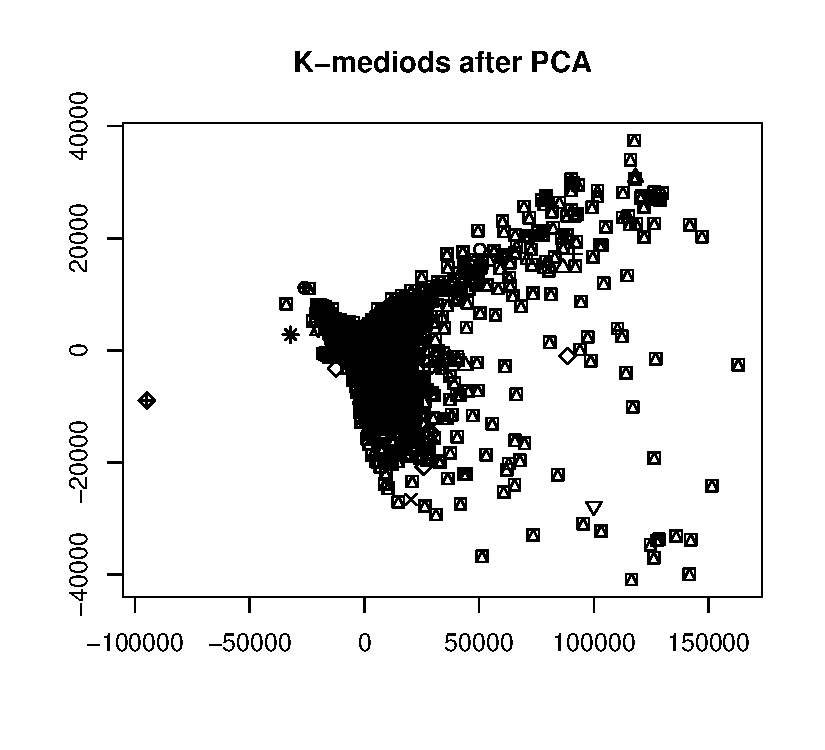
\includegraphics[width=\maxwidth]{figure/minimal-Problem_29} 

}


\begin{kframe}\begin{alltt}
\hlcom{# Comment: Still not good, I don't think PCA is helpful in}
\hlcom{# this case or we need to figure out a combination of PCs to}
\hlcom{# reflect clustering.}
\hlstd{diss_kpca} \hlkwb{<-} \hlkwd{dist}\hlstd{(}\hlkwd{t}\hlstd{(}\hlkwd{rotated}\hlstd{(kp_cancer)))}
\hlstd{kmedoids_kpca} \hlkwb{<-} \hlkwd{pam}\hlstd{(diss_kpca,} \hlnum{14}\hlstd{,} \hlkwc{do.swap} \hlstd{=} \hlnum{FALSE}\hlstd{)}
\hlkwd{plot}\hlstd{(}\hlkwd{rotated}\hlstd{(kp_cancer),} \hlkwc{pch} \hlstd{= kmedoids_kpca}\hlopt{$}\hlstd{cluster,} \hlkwc{xlab} \hlstd{=} \hlstr{""}\hlstd{,}
    \hlkwc{ylab} \hlstd{=} \hlstr{""}\hlstd{,} \hlkwc{main} \hlstd{=} \hlstr{"K-mediods after kernel PCA"}\hlstd{)}
\end{alltt}
\end{kframe}

{\centering 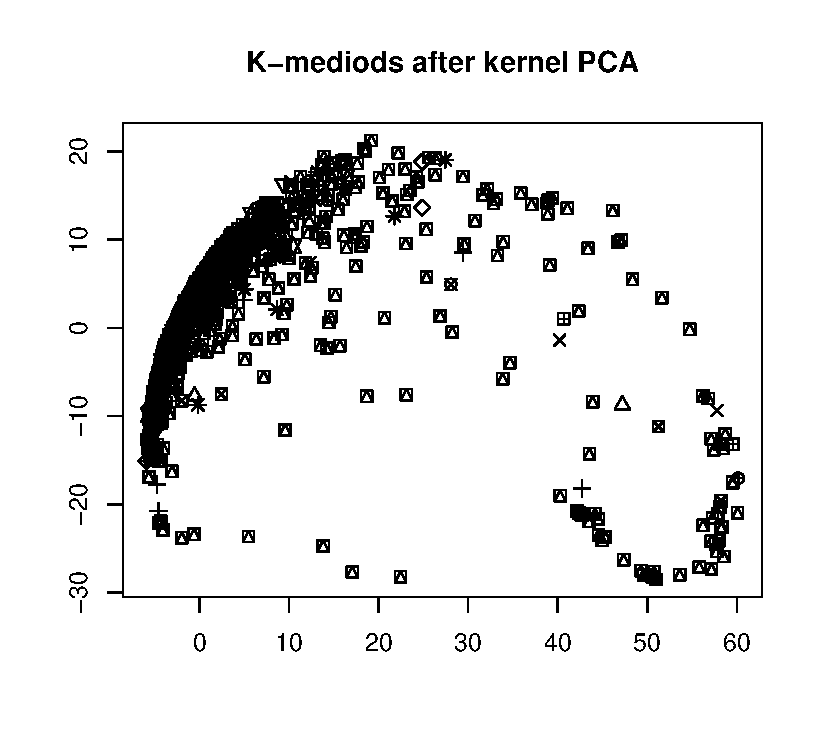
\includegraphics[width=\maxwidth]{figure/minimal-Problem_210} 

}


\begin{kframe}\begin{alltt}
# Comment: Probably it is due to the lack of useful genes or
# it is due to the fact that the principal component needs to
# be further revised in this case, we cannot cluter out the
# points.
\end{alltt}
\end{kframe}
\end{knitrout}

\end{document}
